% !TeX program = pdflatex
\documentclass[border=6pt]{standalone}
\usepackage{tikz}
\usetikzlibrary{arrows.meta, positioning, calc}

\definecolor{MediumRed}{rgb}{0.925, 0.345, 0.345}
\definecolor{MediumGreen}{rgb}{0.37, 0.7, 0.66}
\definecolor{MediumBlue}{rgb}{0.015, 0.315, 0.45}
\definecolor{DarkBlue}{rgb}{0.05, 0.15, 0.35}

\begin{document}
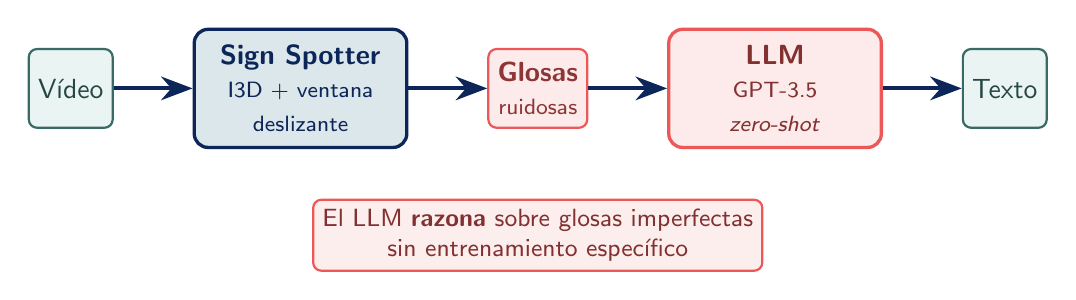
\begin{tikzpicture}[
    font=\sffamily,
    stage/.style={draw=DarkBlue, very thick, rounded corners=5pt,
        fill=MediumBlue!14, text=DarkBlue, align=center,
        minimum width=2.7cm, minimum height=1.5cm},
    data/.style={draw=MediumGreen!60!black, thick, rounded corners=3pt,
        fill=MediumGreen!14, text=MediumGreen!40!black, align=center,
        minimum height=1.0cm},
    flow/.style={-{Stealth[length=4mm]}, line width=1.4pt, DarkBlue},
]

\node[data] (vid) {Vídeo};
\node[stage, right=1.0cm of vid] (spot)
    {\textbf{Sign Spotter}\\\footnotesize I3D + ventana\\\footnotesize deslizante};
\node[data, right=1.0cm of spot, draw=MediumRed, fill=MediumRed!12,
      text=MediumRed!60!black] (gloss)
    {\textbf{Glosas}\\\footnotesize ruidosas};
\node[stage, right=1.0cm of gloss, draw=MediumRed, fill=MediumRed!12,
      text=MediumRed!55!black] (llm)
    {\textbf{LLM}\\\footnotesize GPT-3.5\\\footnotesize \textit{zero-shot}};
\node[data, right=1.0cm of llm] (txt) {Texto};

\foreach \a/\b in {vid/spot, spot/gloss, gloss/llm, llm/txt} \draw[flow] (\a)--(\b);

% mensaje clave
\coordinate (mid) at ($(vid)!0.5!(txt)$);
\node[draw=MediumRed, thick, rounded corners=3pt, fill=MediumRed!10,
      text=MediumRed!55!black, font=\sffamily\small, align=center,
      below=1.4cm of mid]
    {El LLM \textbf{razona} sobre glosas imperfectas\\ sin entrenamiento específico};% $\rightarrow$ \textbf{resiliencia}};

\end{tikzpicture}
\end{document}
